\documentclass[14pt]{extbook}
\usepackage{multicol, enumerate, enumitem, hyperref, color, soul, setspace, parskip, fancyhdr} %General Packages
\usepackage{amssymb, amsthm, amsmath, bbm, latexsym, units, mathtools} %Math Packages
\everymath{\displaystyle} %All math in Display Style
% Packages with additional options
\usepackage[headsep=0.5cm,headheight=12pt, left=1 in,right= 1 in,top= 1 in,bottom= 1 in]{geometry}
\usepackage[usenames,dvipsnames]{xcolor}
\usepackage{dashrule}  % Package to use the command below to create lines between items
\newcommand{\litem}[1]{\item#1\hspace*{-1cm}\rule{\textwidth}{0.4pt}}
\pagestyle{fancy}
\lhead{Progress Quiz 8}
\chead{}
\rhead{Version A}
\lfoot{4553-3922}
\cfoot{}
\rfoot{Fall 2020}
\begin{document}

\begin{enumerate}
\litem{
Solve the quadratic equation below. Then, choose the intervals that the solutions $x_1$ and $x_2$ belong to, with $x_1 \leq x_2$.\[ 15x^{2} +2 x -24 = 0 \]\begin{enumerate}[label=\Alph*.]
\item \( x_1 \in [-1.89, -1.28] \text{ and } x_2 \in [1.15, 1.23] \)
\item \( x_1 \in [-2.76, -2.55] \text{ and } x_2 \in [0.53, 0.88] \)
\item \( x_1 \in [-0.98, 0.53] \text{ and } x_2 \in [2.28, 2.71] \)
\item \( x_1 \in [-21.62, -18.51] \text{ and } x_2 \in [17.82, 18.16] \)
\item \( x_1 \in [-4.04, -3.9] \text{ and } x_2 \in [0, 0.41] \)

\end{enumerate} }
\litem{
Solve the quadratic equation below. Then, choose the intervals that the solutions $x_1$ and $x_2$ belong to, with $x_1 \leq x_2$.\[ 25x^{2} +75 x + 54 = 0 \]\begin{enumerate}[label=\Alph*.]
\item \( x_1 \in [-2.5, -1.77] \text{ and } x_2 \in [-1.37, -1.07] \)
\item \( x_1 \in [-9.43, -8.89] \text{ and } x_2 \in [-0.25, -0.24] \)
\item \( x_1 \in [-6.31, -3.63] \text{ and } x_2 \in [-0.47, -0.39] \)
\item \( x_1 \in [-4.09, -3.14] \text{ and } x_2 \in [-0.72, -0.49] \)
\item \( x_1 \in [-45.41, -44.02] \text{ and } x_2 \in [-30.12, -29.73] \)

\end{enumerate} }
\litem{
Factor the quadratic below. Then, choose the intervals that contain the constants in the form $(ax+b)(cx+d); b \leq d.$\[ 36x^{2} +53 x + 10 \]\begin{enumerate}[label=\Alph*.]
\item \( a \in [25.3, 29.5], \hspace*{5mm} b \in [-2, 6], \hspace*{5mm} c \in [-0.6, 2], \text{ and } \hspace*{5mm} d \in [-3, 9] \)
\item \( a \in [8, 9.6], \hspace*{5mm} b \in [-2, 6], \hspace*{5mm} c \in [2.1, 4.8], \text{ and } \hspace*{5mm} d \in [-3, 9] \)
\item \( a \in [-0.4, 1.4], \hspace*{5mm} b \in [7, 10], \hspace*{5mm} c \in [-0.6, 2], \text{ and } \hspace*{5mm} d \in [43, 50] \)
\item \( a \in [3.4, 4.7], \hspace*{5mm} b \in [-2, 6], \hspace*{5mm} c \in [7.6, 10.2], \text{ and } \hspace*{5mm} d \in [-3, 9] \)
\item \( \text{None of the above.} \)

\end{enumerate} }
\litem{
Graph the equation below.\[ f(x) = -(x-1)^2 + 11 \]\begin{enumerate}[label=\Alph*.]
\begin{multicols}{2}\item 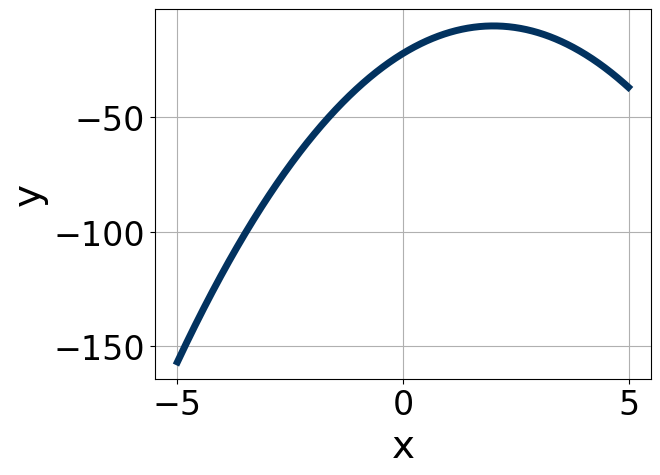
\includegraphics[width = 0.3\textwidth]{../Figures/quadraticEquationToGraphCopyAA.png}\item 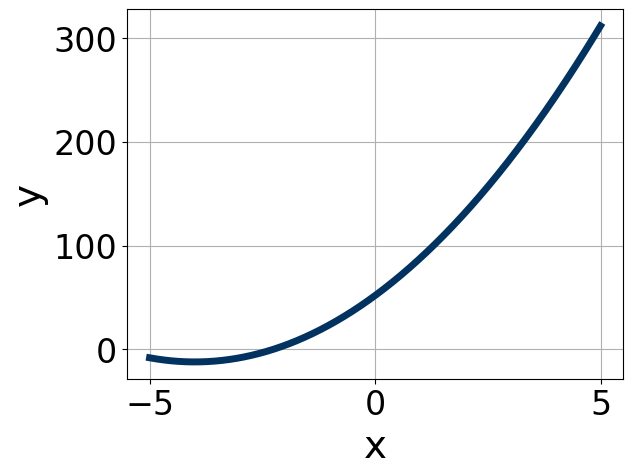
\includegraphics[width = 0.3\textwidth]{../Figures/quadraticEquationToGraphCopyBA.png}\item 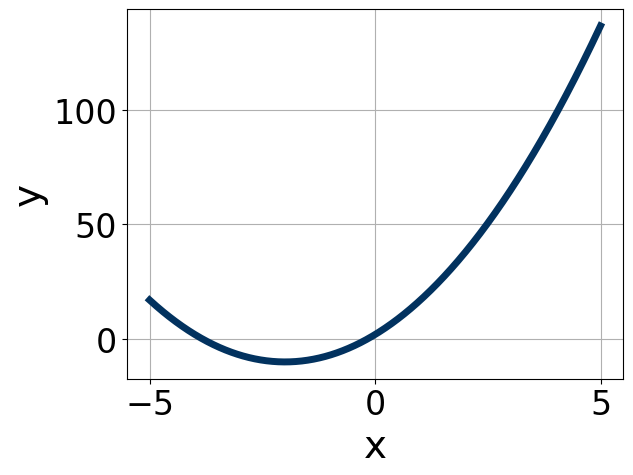
\includegraphics[width = 0.3\textwidth]{../Figures/quadraticEquationToGraphCopyCA.png}\item 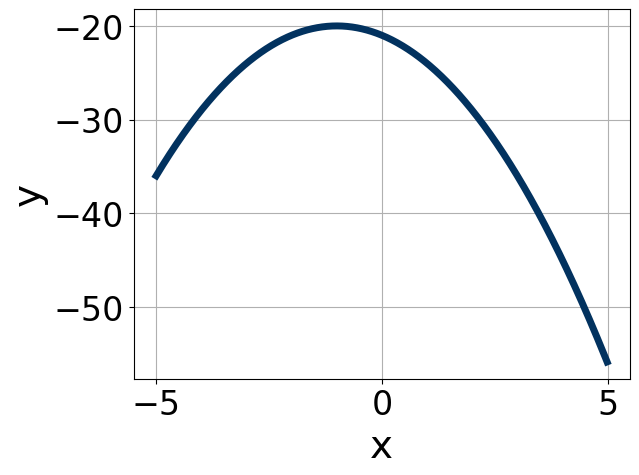
\includegraphics[width = 0.3\textwidth]{../Figures/quadraticEquationToGraphCopyDA.png}\end{multicols}\item None of the above.
\end{enumerate} }
\litem{
Solve the quadratic equation below. Then, choose the intervals that the solutions belong to, with $x_1 \leq x_2$ (if they exist).\[ 13x^{2} +7 x -7 = 0 \]\begin{enumerate}[label=\Alph*.]
\item \( x_1 \in [-20.95, -20.13] \text{ and } x_2 \in [19.3, 21.3] \)
\item \( x_1 \in [-13.84, -13.58] \text{ and } x_2 \in [6.5, 8.1] \)
\item \( x_1 \in [-0.6, -0.26] \text{ and } x_2 \in [0.6, 3.2] \)
\item \( x_1 \in [-1.11, -0.73] \text{ and } x_2 \in [-0.5, 0.8] \)
\item \( \text{There are no Real solutions.} \)

\end{enumerate} }
\litem{
Solve the quadratic equation below. Then, choose the intervals that the solutions belong to, with $x_1 \leq x_2$ (if they exist).\[ -12x^{2} -13 x -2 = 0 \]\begin{enumerate}[label=\Alph*.]
\item \( x_1 \in [-0.4, 0.4] \text{ and } x_2 \in [0.7, 2] \)
\item \( x_1 \in [-1.3, 0] \text{ and } x_2 \in [-0.7, 0.1] \)
\item \( x_1 \in [-9.2, -7.9] \text{ and } x_2 \in [6.2, 8.7] \)
\item \( x_1 \in [2, 3.6] \text{ and } x_2 \in [10, 11.9] \)
\item \( \text{There are no Real solutions.} \)

\end{enumerate} }
\litem{
Write the equation of the graph presented below in the form $f(x)=ax^2+bx+c$, assuming  $a=1$ or $a=-1$. Then, choose the intervals that $a, b,$ and $c$ belong to.
\begin{center}
    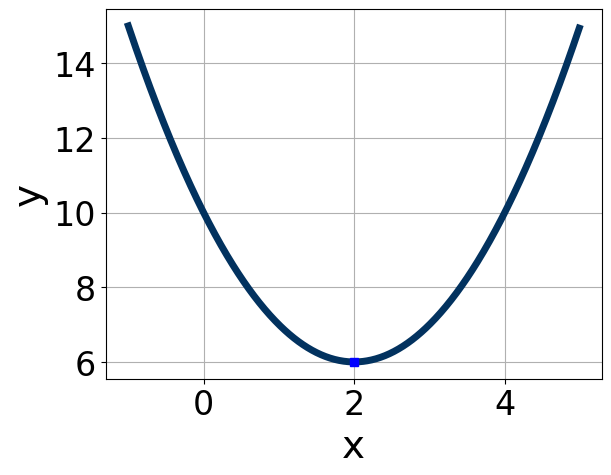
\includegraphics[width=0.5\textwidth]{../Figures/quadraticGraphToEquationA.png}
\end{center}
\begin{enumerate}[label=\Alph*.]
\item \( a \in [0, 2], \hspace*{5mm} b \in [-5, 0], \text{ and } \hspace*{5mm} c \in [7, 11] \)
\item \( a \in [0, 2], \hspace*{5mm} b \in [-5, 0], \text{ and } \hspace*{5mm} c \in [0, 2] \)
\item \( a \in [-1, 0], \hspace*{5mm} b \in [-5, 0], \text{ and } \hspace*{5mm} c \in [0, 2] \)
\item \( a \in [0, 2], \hspace*{5mm} b \in [1, 5], \text{ and } \hspace*{5mm} c \in [7, 11] \)
\item \( a \in [-1, 0], \hspace*{5mm} b \in [1, 5], \text{ and } \hspace*{5mm} c \in [0, 2] \)

\end{enumerate} }
\litem{
Factor the quadratic below. Then, choose the intervals that contain the constants in the form $(ax+b)(cx+d); b \leq d.$\[ 24x^{2} +38 x + 15 \]\begin{enumerate}[label=\Alph*.]
\item \( a \in [0.76, 1.39], \hspace*{5mm} b \in [15, 27], \hspace*{5mm} c \in [-0.34, 1.43], \text{ and } \hspace*{5mm} d \in [13, 21] \)
\item \( a \in [3.16, 4.1], \hspace*{5mm} b \in [2, 7], \hspace*{5mm} c \in [5.71, 7.6], \text{ and } \hspace*{5mm} d \in [3, 11] \)
\item \( a \in [1.31, 2.88], \hspace*{5mm} b \in [2, 7], \hspace*{5mm} c \in [10.56, 13.74], \text{ and } \hspace*{5mm} d \in [3, 11] \)
\item \( a \in [7.73, 8.76], \hspace*{5mm} b \in [2, 7], \hspace*{5mm} c \in [2.39, 3.08], \text{ and } \hspace*{5mm} d \in [3, 11] \)
\item \( \text{None of the above.} \)

\end{enumerate} }
\litem{
Write the equation of the graph presented below in the form $f(x)=ax^2+bx+c$, assuming  $a=1$ or $a=-1$. Then, choose the intervals that $a, b,$ and $c$ belong to.
\begin{center}
    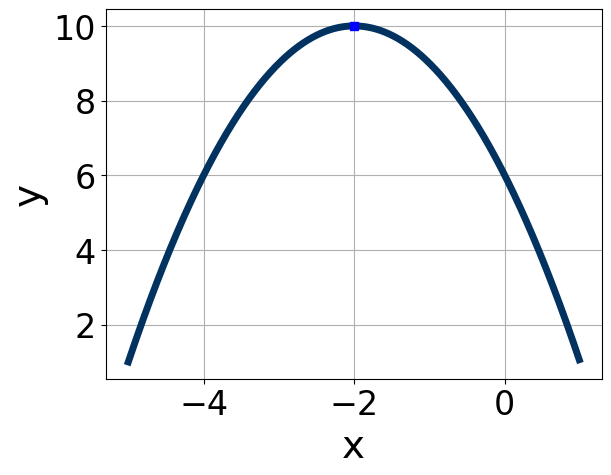
\includegraphics[width=0.5\textwidth]{../Figures/quadraticGraphToEquationCopyA.png}
\end{center}
\begin{enumerate}[label=\Alph*.]
\item \( a \in [0, 3], \hspace*{5mm} b \in [5, 10], \text{ and } \hspace*{5mm} c \in [21, 24] \)
\item \( a \in [-1, 0], \hspace*{5mm} b \in [5, 10], \text{ and } \hspace*{5mm} c \in [-10, -6] \)
\item \( a \in [0, 3], \hspace*{5mm} b \in [-11, -3], \text{ and } \hspace*{5mm} c \in [21, 24] \)
\item \( a \in [-1, 0], \hspace*{5mm} b \in [-11, -3], \text{ and } \hspace*{5mm} c \in [-10, -6] \)
\item \( a \in [0, 3], \hspace*{5mm} b \in [5, 10], \text{ and } \hspace*{5mm} c \in [7, 12] \)

\end{enumerate} }
\litem{
Graph the equation below.\[ f(x) = -(x-4)^2 - 11 \]\begin{enumerate}[label=\Alph*.]
\begin{multicols}{2}\item 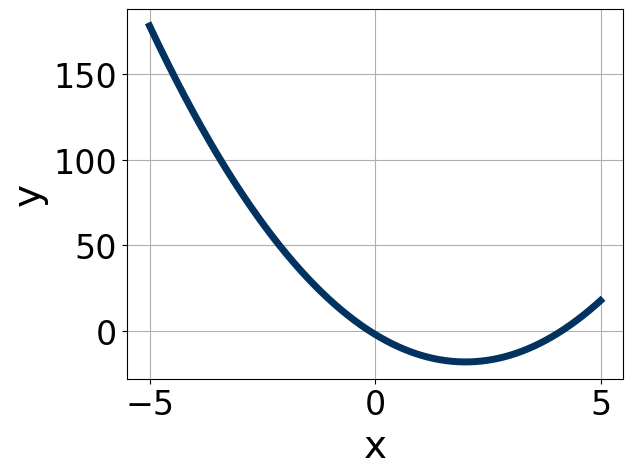
\includegraphics[width = 0.3\textwidth]{../Figures/quadraticEquationToGraphAA.png}\item 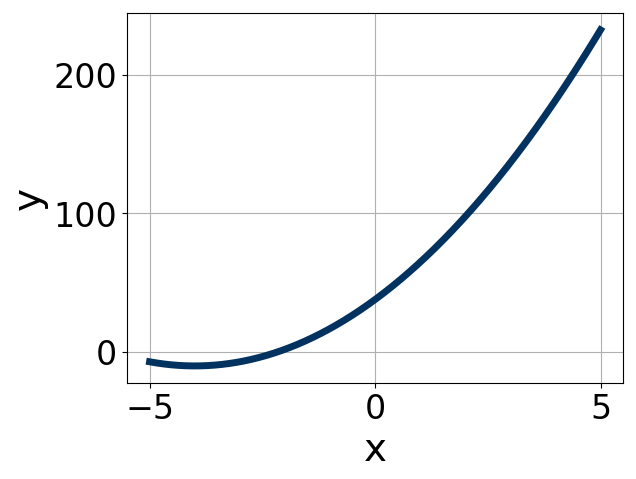
\includegraphics[width = 0.3\textwidth]{../Figures/quadraticEquationToGraphBA.png}\item 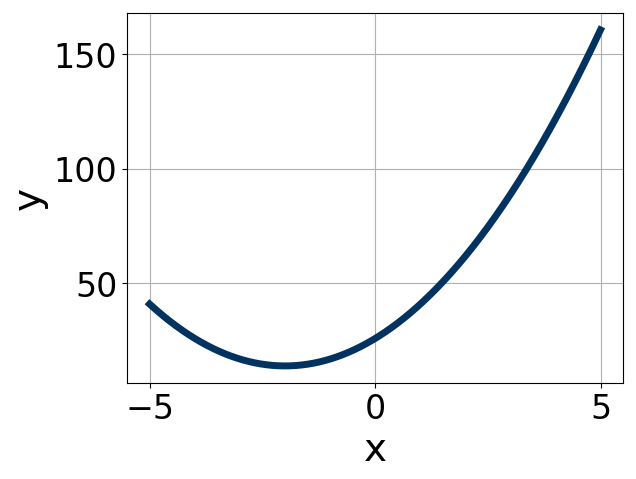
\includegraphics[width = 0.3\textwidth]{../Figures/quadraticEquationToGraphCA.png}\item 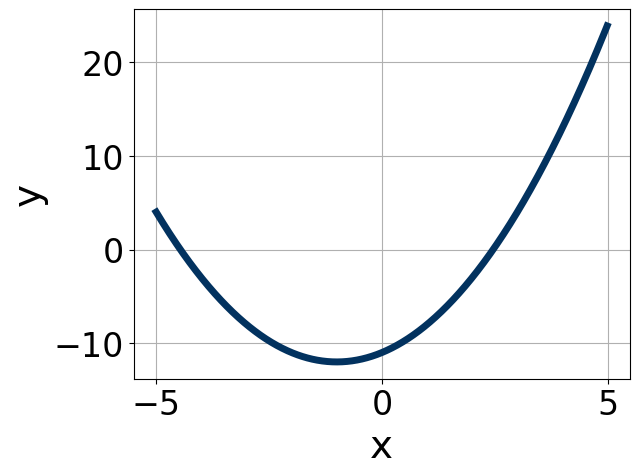
\includegraphics[width = 0.3\textwidth]{../Figures/quadraticEquationToGraphDA.png}\end{multicols}\item None of the above.
\end{enumerate} }
\end{enumerate}

\end{document}